\section{Shortbread}

\begin{itemize}
	\item 125g/4oz butter
	\item 55g/2oz caster sugar, plus extra to finish
	\item 180g/6oz plain flour
\end{itemize}

\subsection{Method}

\begin{enumerate}
\item Heat the oven to 190C/375F/Gas 5.
\item Beat the butter and the sugar together until smooth.
\item Stir in the flour to get a smooth paste. Turn on to a work surface and gently roll out until the paste is 1cm/in thick.
\item Cut into rounds or fingers and place onto a baking tray. Sprinkle with caster sugar and chill in the fridge for 20 minutes.
\item Bake in the oven for 15-20 minutes, or until pale golden-brown. Set aside to cool on a wire rack.
\end{enumerate}

\begin{figure}[h]
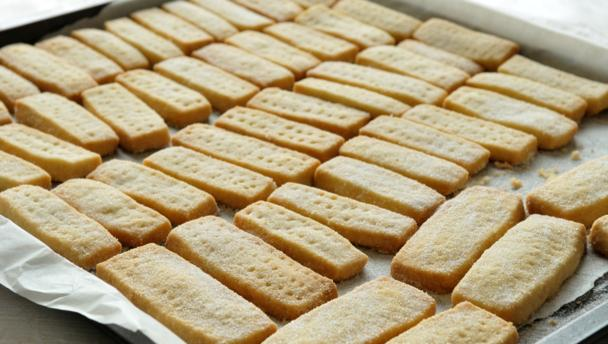
\includegraphics[width=8cm]{shortbread}
\caption{this is a picture of shortbread}
\end{figure}
